\documentclass{acm_proc_article-sp}
\usepackage{algpseudocode}
\usepackage{verbatim}
\usepackage{microtype}
\usepackage{enumerate}
\usepackage{enumitem}
\usepackage{epsfig}
\usepackage{algorithmicx}
\usepackage{algorithm}
\usepackage{algpseudocode}

\renewcommand{\vec}[1]{\mathbf{#1}}

\begin{document}

\title{A Comparative Study of the Echo State Networks}

\numberofauthors{2}
\author{
\alignauthor
Rob Argue\\
       \affaddr{University of Maryland}\\
       \affaddr{Department of Computer Science}\\
       \email{rargue@cs.umd.edu}
\alignauthor
Joshua Bradley\\
       \affaddr{University of Maryland}\\
       \affaddr{Department of Computer Science}\\
       \email{jgbrad1@cs.umd.edu}
}

\date{9 May 2013}

\maketitle
\begin{abstract}
In this study, we compare the performance and behavior of an echo state network (ESN) to the Elman recurrent neural network architecture when applied to the task of nonlinear time series forecasting. To provide a representative baseline in our study, we also give performance comparisons to a feedforward network as well. We will describe several benchmark tests used and provide a discussion of the results. We found that the ESN perfomed best on non-featured time series, and was resiliant to data with missing entries. While the ESN perfomed somewhat worse on some tasks than the Elman net, it ran much quicker and with higher consistancy.
\end{abstract}

\section{Introduction}
Recurrent Neural Networks (RNNs) have been shown to be effective function approximators in time series prediction. One of the disadvantages to applying RNNs to various prediction tasks though is the increased computational cost required to train such networks to a sufficient error threshold. This is due to the network architecture design, in which every node in the hidden layer(s) is conventionally considered to be fully inter-layer connected (i.e. Elman networks, Jordan networks).

Recently, Echo State Networks (ESNs) have been shown to be quite effective at similar tasks, yet not require such great computational cost. They differ in comparison to many other well known RNN architectures like the Elman and Jordan nets, in that the weights of output neurons are the only aspect of the network that can be learned/changed. In this study, we compare the performance and behavior of ESNs to the Elman recurrent neural network architecture. We also provide performance comparisons of the ESN against a feedforward network in an attempt to establish some sense of a \emph{baseline}, which will be used as a discussion point in several of the experiments performed. Our initial expectation of these experiments was that the ESN would perform best on the Mackey-Glass data and worst on the power consumption data. Our report is outlined as follows. In section 2, we give an in-depth discussion of the data sets used and why they were of particular interest to our study. In section 3, a formal description of the particular ESN architecture used in our study is given. Section 4 describes the experimental setup of various tests and discusses results, some of which were unexpected. With section 5, we conclude our report with a short discussion as to why we believe we were able to obtain some of the results presented.

\section{Data}
Selection of the dataset is very important in our study. To ensure a fair comparison of the echo state network and other RNN architectures when applied to time series forecasting, datasets exhibiting specific traits must be chosen. The traits we have chosen to base data selection on include
\begin{itemize}
\item Degree of periodicity - For example, a dataset of household electricity consumption would be expected to exhibit reasonably normal daily periodic patterns while a dataset of certain stock prices may be expected to exhibit annual periodic behavior.
\item Amount of bias/variance within the data - For example, stock pricing depends on a large number of factors in the market to be considered, thus it is expected to exhibit a greater amount of variance and bias vs. a dataset of daily household electricity consumption.
\item Noise - we are interested in using dynamic time series datasets that can provide us varying levels of noise at both extremes, from no noise at all to dealing with large portions of missing data. This will help us to evaluate the ESNs ability to recreate a time series signal and study how performance degradation is effected.
\end{itemize}
Three data sets were used for each of the experiments described in section 4. The time delay differential Mackey-Glass equation,
\begin{equation*}
\frac{dx}{dt} = \beta \frac{x_\tau}{1+x_{\tau}^\eta} - \gamma x \text{  for  } \gamma, \beta, \eta \ge 0
\end{equation*}
was used to generate the first set of data, using a time delay of $\tau = 17$ and letting $\eta = 10$, $\beta = 0.2$, and $\gamma = 0.1$. When $\tau = 17$, this produces a mildly chaotic time series with no additional features considered. The use of a mathematically-based time series allowed us to generate a dataset with no noise present.

As a second dataset, stock market pricing \cite{industryportfolio} was chosen as a good representation of chaotic data with potentially highly varying dynamics. Within this dataset, pricing of multiple stock portfolios was used as ''features'' to predict another selected target portfolio. For the purpose of the experiments in this report, we chose the finance sector portfolio price as the target, and all other sectors were utilized as features.

For a third dataset, records of household power consumption \cite{Hebrail+Berard:2012} were selected in our attempt to find a dataset with more periodic behavior but with what we found to include noise and much missing data. For the purposes of our report, all datasets were preprocessed and normalized within the range of $[-1,1]$.

\section{Methodology}

For the ESN, we decided to use the following structure.
\begin{figure}[here]
\begin{center}
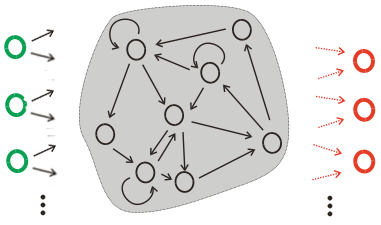
\includegraphics[scale=0.35]{ESNStructure.png}
\caption{ESN architecture}
\end{center}
\label{fig:esn_structure}
\end{figure}
There exist many variants of the ESN, however for the best comparison of the ESN and Elman networks, we felt it would be most appropriate to employ a design where feedback connections exist only within the reservoir. For a legitimate comparison to Jordan networks, one would need to provide feedback connections from the output back into the reservoir. To account for the potential occurrence of slow dynamics, the reservoir is made up of leaky integrator neurons \cite{Jaeger1}. The ESN in this study was constructed and trained in the following manner.
\begin{enumerate}
\item Generate an untrained dynamical reservoir network by computing random values for the weight matrices $\vec{W}^{in}$, $\vec{W}$, and $\vec{W}^{back}$.
\item Ensure the reservoir has the echo state property and displays mutually different dynamics upon excitement. This was done by populating $\vec{W}$ with random values in the range $[-1, 1]$ and setting
\begin{eqnarray*}
W = \frac{\alpha}{|\lambda_{max}|} W
\end{eqnarray*}
where $\lambda$ is the eigenvalue of $W$ and $\alpha \in (0,1)$ is defined as the \emph{spectral radius}.
\item Arbitrarily initialize the network state $\vec{x}(0)$.
\item For training time $t = 0 \ldots T$, run each input pattern $\vec{u}(t)$ and target output $\vec{d}(t)$ through the ESN, updating the network by
\begin{eqnarray*}
\vec{x}(t+1) = (1-k)\vec{x}(t) + k \vec{f}(\vec{W}^{in} \vec{u}(t+1) + \vec{W} \vec{x}(t))
\end{eqnarray*}
where f is any sigmoidal activation function and $k \in [0, 1]$ is some defined leak rate. For our experiments, we let f = $\tanh$. If trained output-to-reservoir connections are used, then updating the network would require
\begin{eqnarray*}
\vec{x}(t+1) = (1-k)\vec{x}(t) + k \vec{f}(\vec{W}^{in} \vec{u}(t+1) + \vec{W} \vec{x}(t) + \vec{W}^{back} \vec{d}(t))
\end{eqnarray*}
\item Once a particular amount of \emph{washout} time has passed, begin collecting network states in a matrix $\vec{C}$ row-by-row where each row is a concatenation of the vectors $(\vec{u}(t), \vec{x}(t))$. Also store the target output into each row of a matrix T as $\vec{f}^{-1}(\vec{d}(t))$. In our case, this was $\tanh^{-1}(\vec{d}(t))$.
\item To calculate $\vec{W}^{out}$, the final learning step is to compute the pseudoinverse of the matrices $\vec{C}$ and $\vec{T}$.
\begin{eqnarray*}
(\vec{W}^{out})^\top = \vec{C}^{-1} \vec{T}
\end{eqnarray*}
\end{enumerate}

After training, to test for time series predictions, all one must do is run the following update equations
\begin{eqnarray*}
\vec{x}(t+1) &=& \vec{f}(\vec{W}^{in} \vec{u}(t+1) + \vec{W} \vec{x}(t)) \\
\vec{y}(t+1) &=& \vec{f}(\vec{W}^{out} (\vec{u}(t+1), \vec{x}(t+1), \vec{y}(t))) \\
\end{eqnarray*}
When feedback connections from the output to the reservoir are considered, the update equation for the network state becomes
\begin{eqnarray*}
\vec{x}(t+1) = \vec{f}(\vec{W}^{in} \vec{u}(t+1) + \vec{W} \vec{x}(t) + \vec{W}^{back} \vec{y}(t))
\end{eqnarray*}

\section{Experiments}
For the analysis of our ESN, three experiments were run. The initial experiment was parameter optimization for three paremters of the ESN, and sought to explore the effects of network architecture and learning rule parameters on the performance of the model. In all experiments, performance was measured as the mean square error (MSE) of ESN output vs. actual test immediately following the training data. Lastly a run-time comparison of the networks was conducted using the power consumption data set.

Parameter optimization for the ESN was run over the following parameters: \emph{leak rate}, \emph{reservoir size}, \emph{spectral radius}, and \emph{forget size}. For each data set each parameter was varied independently of the others, which were held at default values of
\begin{align*}
\text{leak rate} &= 0.5 \\
\text{reservoir size} &= 100 \\
\text{spectral radius} &= 0.5 \\
\text{forget size} &= 100
\end{align*}
\begin{center}
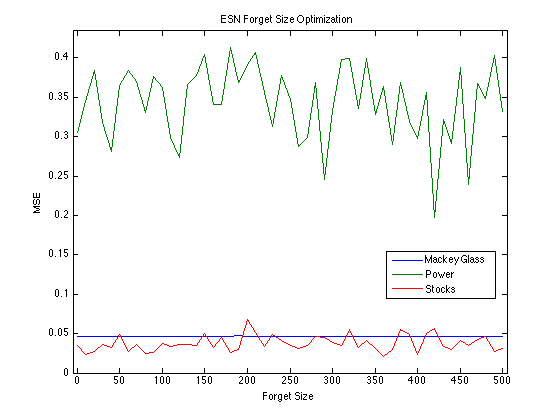
\includegraphics[scale=0.45]{ForgetSizeOptimization.png}
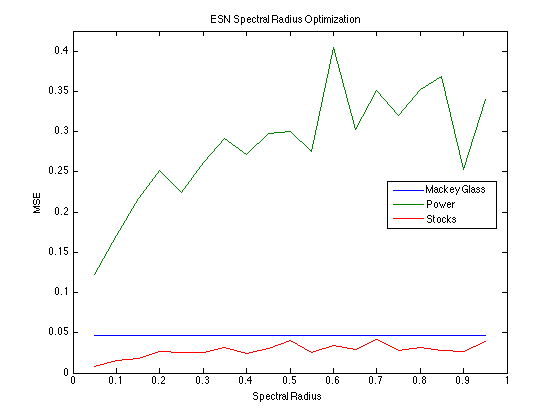
\includegraphics[scale=0.45]{SpectralRadiusOptimization.png}
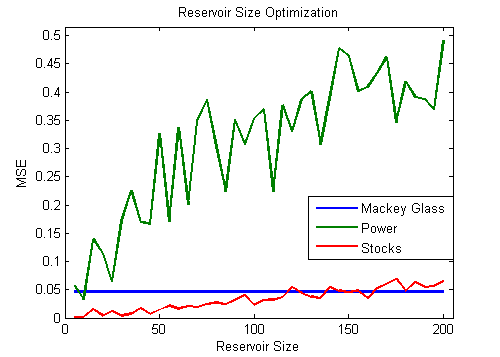
\includegraphics[scale=0.45]{ReservoirSizeOptimization.png}
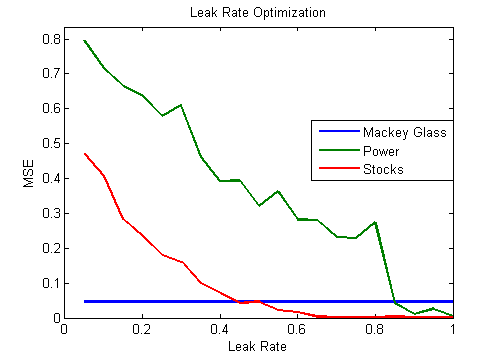
\includegraphics[scale=0.45]{LeakRateOptimization.png}
\end{center}

For all of the parameters, the Mackey-Glass performance remained constant, which is consistent with what we saw when run on other network architectures. This behavior is likely due to the mild chaotic behavior of the data when $\tau = 17$ in the original equation. Setting $\tau = 30$ would have exhibited a more wildly chaotic attractor. Varying \emph{forget size} appeared to have little to no effect on the performance of the ESN. The original expectation was that there would be a higher MSE when \emph{forget size} $\approx 0$, which would then quickly drop to a stable value as \emph{forget size} grew larger. The ESN tended to perform better with a smaller \emph{spectral radius}. Most surprising was that \emph{reservoir size} had a positive correlation with error, which is the opposite of expectation.  The decay of error with a higher \emph{leak rate} matched what we expected to happen.  Possible explanations for these results not matching our original hypothesized results could be in our implementation of the ESN. For $k$ features in a dataset, we define the number of input nodes into the ESN to be $k$ as well. Further analysis of the input weights $W^{in}$ must be done but it is known that large absolute $W^{in}$ can imply that the ESN is strongly influenced by input while a small absolute $W^{in}$ implies the network state is only slightly excited around the resting state \cite{Jaeger2}.

In the second experiment we compared our ESN to other, commercially available neural networks. In particular we compared it to a feed-forward network as a control, and to an Elman network as an example of another type of recurrent architecture. Matlab's Neural Network Toolbox was used for these networks. All three of the comparison networks were trained using RProp, and a best of three runs approach was taken in the attempt to minimize the effect of outliers. We varied the size of the hidden layer (analagous to the ''reservoir'' in the case of our ESN) for some variety in architecture. The ESN used parameters optimized to each data set, while the other networks used default Matlab parameters in the interest of time.

\begin{center}
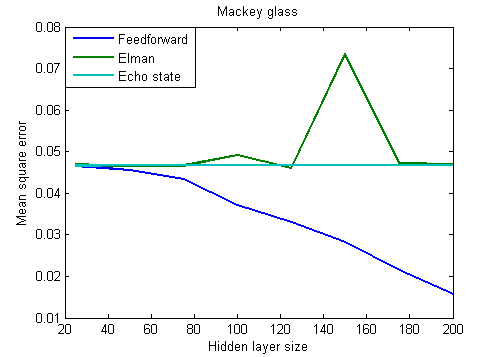
\includegraphics[scale=0.7]{mackey_plot.png}
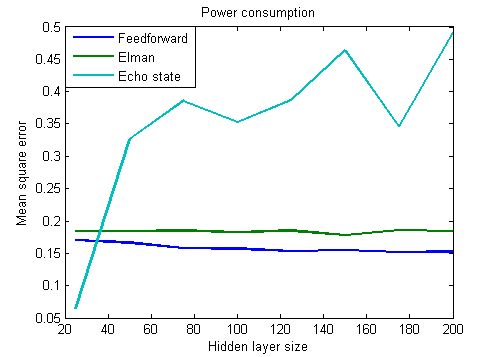
\includegraphics[scale=0.7]{power_plot.png}
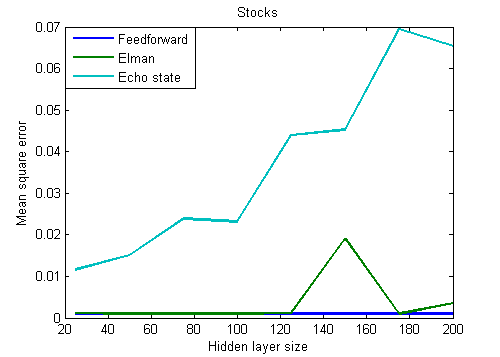
\includegraphics[scale=0.7]{stocks_plot.png}
\end{center}

The ESN performed best on the Mackey-Glass dataset, proving to be approximately equal to the Elman net in terms of MSE, though with a significantly less variance across runs, which matched with our expectations. For the power consumption dataset, the ESN performed somewhat poorer than the feed-forward and Elman net, with approximately double the error. On the stocks dataset the ESN performed significantly worse than the feedforward and Elman nets. This seems to indicate a general trend that the ESN performs more comparably on datasets which have fewer features, and instead tend to be more pure functions of time. Once again, a closer analysis of the weight connections from the input nodes may yield further insight into this behavior. Contrary to our initial hypothesis, did not seem to perform significantly worse compared to the other networks on the data set with missing data (the power consumption data set). 

The run-time experiment was conducted under the same circumstances as the second experiment, however was only run on the power data set. The run-time was taken to be the average of three runs.

\begin{center}
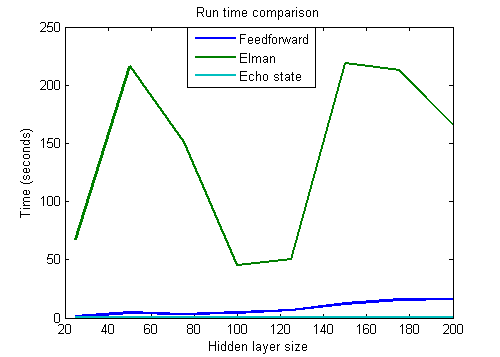
\includegraphics[scale=0.7]{time_plot.png}
\end{center}

The ESN took significantly less time to train, especially with larger reservoir sizes, running orders of magnitude faster than the Elman net, even at a small network size.

\section{Conclusions}
Our current ESN implementation has the ability to have output to reservoir connections, which we felt would be good to include for a comparison to Jordan nets. We were unable to finish experiments involving the Jordan nets in time to be able to conduct a proper comparison, thus it has been left as future work. Additionally, parameter optimization for the Matlab nets could be performed, and other learning methods investigated as well. Currently, our ESN could be adapted to utilize multiple time series as well, and comparisons could be done with those.

In general, we found the ESN to perform reasonably well when compared to other simple recurrent nets. The ESN tended to have somewhat worse performance, especially on many-featured data, but took significantly shorter time to train, and was less prone to getting stuck in local minima, especially when compared to the Elman net.

\bibliographystyle{abbrv}
\bibliography{report_argue_bradley}

\balancecolumns
\end{document}
